
\let\negmedspace\undefined
\let\negthickspace\undefined
\documentclass[journal]{IEEEtran}
\usepackage[a5paper, margin=10mm, onecolumn]{geometry}
% \usepackage{lmodern} % Ensure lmodern is loaded for pdflatex
\usepackage{tikz} % Include TikZ package

\setlength{\headheight}{1cm} % Set the height of the header box
\setlength{\headsep}{0mm}    % Set the distance between the header and text

\usepackage{gvv-book}
\usepackage{gvv}
\usepackage{cite}
\usepackage{amsmath,amssymb,amsfonts,amsthm}
\usepackage{algorithmic}
\usepackage{graphicx}
\usepackage{textcomp}
\usepackage{xcolor}
\usepackage{txfonts}
\usepackage{listings}
\usepackage{enumitem}
\usepackage{mathtools}
\usepackage{gensymb}
\usepackage{comment}
\usepackage[breaklinks=true]{hyperref}
\usepackage{tkz-euclide} 
\usepackage{listings}
% \usepackage{gvv}                                        
\def\inputGnumericTable{}                                 
\usepackage[latin1]{inputenc}                                
\usepackage{color}                                            
\usepackage{array}                                            
\usepackage{longtable}                                       
\usepackage{calc}                                             
\usepackage{multirow}                                         
\usepackage{hhline}                                           
\usepackage{ifthen}                                           
\usepackage{lscape}
\usepackage{circuitikz}
\tikzstyle{block} = [rectangle, draw, fill=blue!20, 
    text width=4em, text centered, rounded corners, minimum height=3em]
\tikzstyle{sum} = [draw, fill=blue!10, circle, minimum size=1cm, node distance=1.5cm]
\tikzstyle{input} = [coordinate]
\tikzstyle{output} = [coordinate]

\begin{document}

\bibliographystyle{IEEEtran}
\vspace{3cm}

\title{1.4.12}
\author{ai25tech11037-stalin}
\maketitle
% \newpage
% \bigskip
{\let\newpage\relax\maketitle}

\renewcommand{\thefigure}{\theenumi}
\renewcommand{\thetable}{\theenumi}
\setlength{\intextsep}{10pt} % Space between text and floats

\numberwithin{equation}{enumi}
\numberwithin{figure}{enumi}
\renewcommand{\thetable}{\theenumi}

\textbf{Problem:} \\ 
\\
In what ratio does the point \( P(-4, 6) \) divide the line segment joining the points \( A(-6, 0) \) and \( C(3, -8) \)? 
\\

\solution\\

Given Points
\begin{align*}
\vec{A} &= \myvec{-6 \\ 0}, \quad
\vec{C} =  \myvec{3 \\ -8}, \quad
\vec{P} = \myvec{-4 \\ 6},
\end{align*}

the ratio \( k \) in which \( P \) divides \( AC \) is
\[
k = \frac{(\vec{A} - \vec{P})^T (\vec{P} - \vec{C})}{\|\vec{P} - \vec{C}\|^2}
\]

\[
=\frac{
 \myvec{-6 + 4 \\ 0 - 6}^T 
 \myvec{-4 - 3 \\ 6 + 8}
}{
(-4 - 3)^2 + (6 + 8)^2
}
\]

\[
=\frac{
 \myvec{-2 \\ -6}^T
 \myvec{-7 \\ 14}
}{
(-7)^2 + 14^2
}
\]

Therefore,
\[
k = \frac{-70}{245} = -\frac{2}{7}.
\]

Since \( k = -\frac{2}{7} \), Point \( P \) divides the segment \( AC \) \textbf{externally} in the ratio \( 2 : 7 \).

\begin{figure}
    \centering
    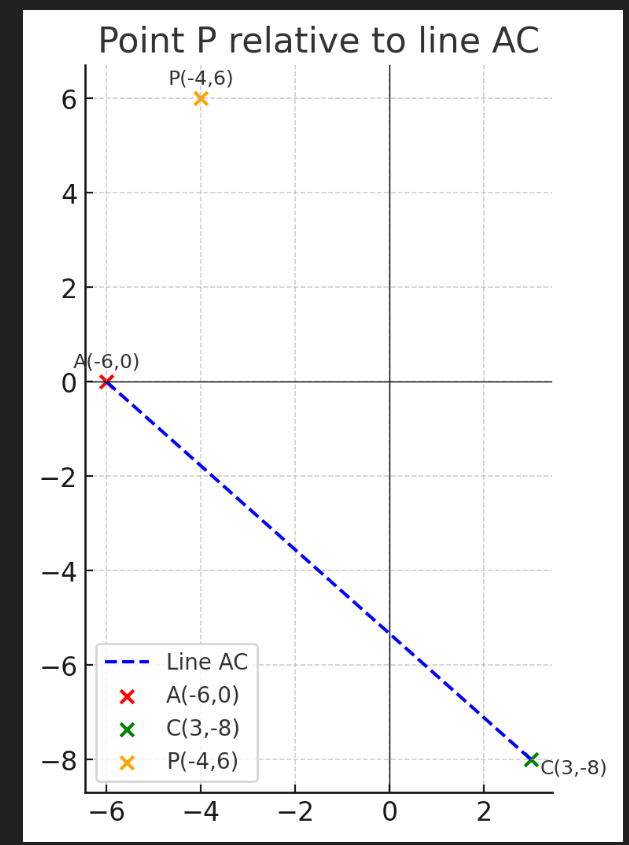
\includegraphics[width=0.3\linewidth]{Fig1.png}
    \caption{Caption}
    \label{fig:placeholder}
\end{figure}

\end{document}
